\section*{Oppgave 4: Lineær manipulering}

Oppgaven som gikk på lineær manipulering var ikke så godt beskrevet i oppgaven, men jeg har tatt utgangspunkt i at det er et positivt eller negativt tall som adderes til den aktuelle komponenten/kanelen på alle punkter i bildet.

Parametrene for å manipulere verdiene i bildet sendes med til frontend som vist i hjelp for denoise.c;

%@input
--lr N  Amount to add to or remove from the R channel (RGB).
--lg N  Amount to add to or remove from the G channel (RGB).
--lb N  Amount to add to or remove from the B channel (RGB).
--lh N  Amount to add to or remove from the H component (HSI).
--ls N  Amount to add to or remove from the S component (HSI).
--li N  Amount to add to or remove from the I component (HSI).
%@

Manipulering av flere kanaler kan gjøres samtidig og all manipulering skjer etter evt. denoising. Ettersom konvertering til/fra HSI er krevende sjekkes det om det skal gjøres manipulering av noen av HSI-komponentene, og evt. konvertering gjøres da. RGB krever ikke noen konvertering ettersom verdiene i arrayet er RGB-verdier.

Det er implementert sjekker for å sørge for at ingen manipulering fører til verdier som er utenfor grensene som gjelder for de ulike komponentene.

\subsection*{Eksempel på lineær manipulering}
\begin{figure}[!h]
\centering

\includegraphics[width=90mm]{disasterbeforecolor}
\caption{Original image}
\end{figure}

\pagebreak

\begin{figure}[!h]
\centering
%@exec
python denoise.py assets/disasterbeforecolor.jpg \
report/images/nw-color-02-5-100-02.jpg --kappa=0.2 --iter=5 --lr=100 --ls=-0.2
%@
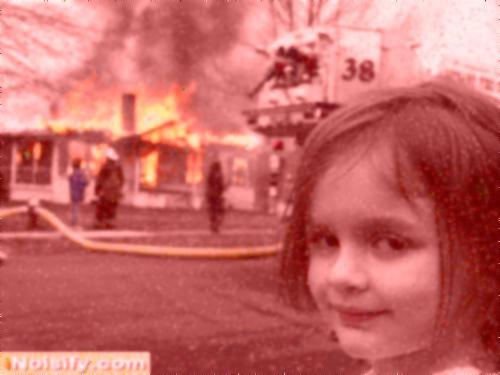
\includegraphics[width=90mm]{nw-color-02-5-100-02}
\caption{Denoised with numpy-weave, kappa=0.2, iter=5, r=100, s=-0.2}
\end{figure}

\pagebreak